\documentclass[mathserif]{beamer}

\setbeamertemplate{frametitle}[default][center]%Centers the frame title.
\setbeamertemplate{navigation symbols}{}%Removes navigation symbols.
\setbeamertemplate{footline}{\raisebox{5pt}{\makebox[\paperwidth]{\hfill\makebox[10pt]{\scriptsize\insertframenumber}}}}
\setbeamertemplate{caption}[numbered]

%\newcommand{\tth}   {\mbox{$\theta$}}
\newcommand{\thh}   {\mbox{$\theta$}}
\newcommand{\su}   {\mbox{$\sigma^2$}}
\newcommand{\so}   {\mbox{$\sigma_0^2$}}
\newcommand{\ko}   {\mbox{$\kappa_0$}}
\newcommand{\no}   {\mbox{$\nu_0$}}
\newcommand{\mo}   {\mbox{$\mu_0$}}
\newcommand{\ti}   {\mbox{$\tilde{x}$}}
\newcommand{\la}   {\mbox{$\lambda$}}
\newcommand{\bx}   {\mbox{$\bm{x}$}}
\newcommand{\bZ}   {\mbox{$\bm{Z}$}}
\newcommand{\bX}   {\mbox{$\bm{X}$}}
\newcommand{\bY}   {\mbox{$\bm{Y}$}}
\newcommand{\bA}   {\mbox{$\bm{A}$}}
\newcommand{\ba}   {\mbox{$\bm{a}$}}
\newcommand{\bb}   {\mbox{$\bm{b}$}}
\newcommand{\bt}   {\mbox{$\bm{t}$}}
\newcommand{\bz}   {\mbox{$\bm{z}$}}
\newcommand{\bw}   {\mbox{$\bm{w}$}}
\newcommand{\bbeta}   {\mbox{$\bm{\beta}$}}

\newcommand{\be}   {\mbox{$\bm{e}$}}
\newcommand{\bu}   {\mbox{$\bm{u}$}}
\newcommand{\bv}   {\mbox{$\bm{v}$}}
\newcommand{\sig}   {\mbox{$\Sigma$}}
\newcommand{\sigx}   {\mbox{$\Sigma_{XX}$}}
\newcommand{\sigxy}   {\mbox{$\Sigma_{XY}$}}
\newcommand{\tr}   {\mbox{$\text{tr}$}}
\newcommand{\ddet}   {\mbox{$\text{det}$}}
\newcommand\independent{\protect\mathpalette{\protect\independenT}{\perp}}
\def\independenT#1#2{\mathrel{\rlap{$#1#2$}\mkern2mu{#1#2}}}

\newcommand{\Expect}[1]{\ensuremath{\mathbf{E}\left[ #1 \right]}}
%\newcommand{\Var}[1]{\ensuremath{\mathrm{Var}\left[ #1 \right]}}
%\newcommand{\Cov}[1]{\ensuremath{\mathrm{Cov}\left[ #1 \right]}}
\newcommand{\MSE}{\ensuremath{\mathrm{MSE}}}
\newcommand{\RSS}{\ensuremath{\mathrm{RSS}}}
\newcommand{\Prob}[1]{\ensuremath{\mathrm{Pr}\left( #1 \right)}}
\newcommand{\ProbEst}[1]{\ensuremath{\widehat{\mathrm{Pr}}\left( #1 \right)}}
\DeclareMathOperator*{\argmin}{argmin} % thanks, wikipedia!
\DeclareMathOperator*{\argmax}{argmax} % thanks, wikipedia!
\DeclareMathOperator*{\sgn}{sgn} % thanks, wikipedia!

\newcommand{\lam}{\lambda}
\newcommand{\bmu}{\bm{\mu}}
%\newcommand{\bx}{\ensuremath{\mathbf{X}}}
\newcommand{\X}{\ensuremath{\mathbf{X}}}
\newcommand{\w}{\ensuremath{\mathbf{w}}}
\newcommand{\h}{\ensuremath{\mathbf{h}}}
\newcommand{\V}{\ensuremath{\mathbf{V}}}
%\newcommand{\tr}{\operatorname{tr}}

%\newcommand{\bx}{\ensuremath{\mathbf{X}}}
%\newcommand{\X}{\ensuremath{\mathbf{x}}}
%\newcommand{\w}{\ensuremath{\mathbf{w}}}
%\newcommand{\h}{\ensuremath{\mathbf{h}}}
%\newcommand{\V}{\ensuremath{\mathbf{v}}}
%\newcommand{\Cov}{\text{Cov}}
%\newcommand{\Var}{\text{Var}}

\DeclareMathOperator{\var}{Var}
\DeclareMathOperator{\cov}{Cov}
\newcommand{\Var}[1]{\ensuremath{\mathrm{Var}\left[ #1 \right]}}
\newcommand{\Cov}[1]{\ensuremath{\mathrm{Cov}\left[ #1 \right]}}


\newcommand{\indep}{\rotatebox{90}{\ensuremath{\models}}}
\newcommand{\notindep}{\not\hspace{-.05in}\indep}







\usepackage{float}
\floatstyle{boxed}
\newfloat{code}{tp}{code}
\floatname{code}{Code Example}
\newcommand{\tth}   {\mbox{$\theta$}}
\newcommand{\thh}   {\mbox{$\theta$}}
\newcommand{\su}   {\mbox{$\sigma^2$}}
\newcommand{\so}   {\mbox{$\sigma_0^2$}}
\newcommand{\ko}   {\mbox{$\kappa_0$}}
\newcommand{\no}   {\mbox{$\nu_0$}}
\newcommand{\mo}   {\mbox{$\mu_0$}}
\newcommand{\ti}   {\mbox{$\tilde{x}$}}
\newcommand{\la}   {\mbox{$\lambda$}}
\newcommand{\bx}   {\mbox{$\bm{x}$}}
\newcommand{\bZ}   {\mbox{$\bm{Z}$}}
\newcommand{\bX}   {\mbox{$\bm{X}$}}
\newcommand{\bY}   {\mbox{$\bm{Y}$}}
\newcommand{\bA}   {\mbox{$\bm{A}$}}
\newcommand{\ba}   {\mbox{$\bm{a}$}}
\newcommand{\bb}   {\mbox{$\bm{b}$}}
\newcommand{\bt}   {\mbox{$\bm{t}$}}
\newcommand{\bz}   {\mbox{$\bm{z}$}}
\newcommand{\bw}   {\mbox{$\bm{w}$}}
\newcommand{\bbeta}   {\mbox{$\bm{\beta}$}}

\newcommand{\be}   {\mbox{$\bm{e}$}}
\newcommand{\bu}   {\mbox{$\bm{u}$}}
\newcommand{\bv}   {\mbox{$\bm{v}$}}
\newcommand{\sig}   {\mbox{$\Sigma$}}
\newcommand{\sigx}   {\mbox{$\Sigma_{XX}$}}
\newcommand{\sigxy}   {\mbox{$\Sigma_{XY}$}}
\newcommand{\tr}   {\mbox{$\text{tr}$}}
\newcommand{\ddet}   {\mbox{$\text{det}$}}
\newcommand\independent{\protect\mathpalette{\protect\independenT}{\perp}}
\def\independenT#1#2{\mathrel{\rlap{$#1#2$}\mkern2mu{#1#2}}}

\newcommand{\Expect}[1]{\ensuremath{\mathbf{E}\left[ #1 \right]}}
%\newcommand{\Var}[1]{\ensuremath{\mathrm{Var}\left[ #1 \right]}}
%\newcommand{\Cov}[1]{\ensuremath{\mathrm{Cov}\left[ #1 \right]}}
\newcommand{\MSE}{\ensuremath{\mathrm{MSE}}}
\newcommand{\RSS}{\ensuremath{\mathrm{RSS}}}
\newcommand{\Prob}[1]{\ensuremath{\mathrm{Pr}\left( #1 \right)}}
\newcommand{\ProbEst}[1]{\ensuremath{\widehat{\mathrm{Pr}}\left( #1 \right)}}
\DeclareMathOperator*{\argmin}{argmin} % thanks, wikipedia!
\DeclareMathOperator*{\argmax}{argmax} % thanks, wikipedia!
\DeclareMathOperator*{\sgn}{sgn} % thanks, wikipedia!

\newcommand{\lam}{\lambda}
\newcommand{\bmu}{\bm{\mu}}
%\newcommand{\bx}{\ensuremath{\mathbf{X}}}
\newcommand{\X}{\ensuremath{\mathbf{X}}}
\newcommand{\w}{\ensuremath{\mathbf{w}}}
\newcommand{\h}{\ensuremath{\mathbf{h}}}
\newcommand{\V}{\ensuremath{\mathbf{V}}}
%\newcommand{\tr}{\operatorname{tr}}

%\newcommand{\bx}{\ensuremath{\mathbf{X}}}
%\newcommand{\X}{\ensuremath{\mathbf{x}}}
%\newcommand{\w}{\ensuremath{\mathbf{w}}}
%\newcommand{\h}{\ensuremath{\mathbf{h}}}
%\newcommand{\V}{\ensuremath{\mathbf{v}}}
%\newcommand{\Cov}{\text{Cov}}
%\newcommand{\Var}{\text{Var}}

\DeclareMathOperator{\var}{Var}
\DeclareMathOperator{\cov}{Cov}
\newcommand{\Var}[1]{\ensuremath{\mathrm{Var}\left[ #1 \right]}}
\newcommand{\Cov}[1]{\ensuremath{\mathrm{Cov}\left[ #1 \right]}}


\newcommand{\indep}{\rotatebox{90}{\ensuremath{\models}}}
\newcommand{\notindep}{\not\hspace{-.05in}\indep}






%\usepackage{fontspec}
%\setmainfont{Tahoma}

%\newcommand{\lam}{\lambda}
%\newcommand{\bmu}{\bm{\mu}}
%%\newcommand{\bx}{\ensuremath{\mathbf{X}}}
%\newcommand{\X}{\ensuremath{\mathbf{x}}}
%\newcommand{\w}{\ensuremath{\mathbf{w}}}
%\newcommand{\h}{\ensuremath{\mathbf{h}}}
%\newcommand{\V}{\ensuremath{\mathbf{v}}}
%\newcommand{\cov}{\text{Cov}}
%\newcommand{\var{\text{Var}}}

%\DeclareMathOperator{\var}{Var}
%\DeclareMathOperator{\cov}{Cov}

%\newcommand{\indep}{\rotatebox{90}{\ensuremath{\models}}}
%\newcommand{\notindep}{\not\hspace{-.05in}\indep}

\usepackage{graphicx} %The mode "LaTeX => PDF" allows the following formats: .jpg  .png  .pdf  .mps
\graphicspath{{./PresentationPictures/}} %Where the figures folder is located
\usepackage{listings}
\usepackage{media9}
\usepackage{movie15}
\addmediapath{./Movies/}

\newcommand{\beginbackup}{
   \newcounter{framenumbervorappendix}
   \setcounter{framenumbervorappendix}{\value{framenumber}}
}
\newcommand{\backupend}{
   \addtocounter{framenumbervorappendix}{-\value{framenumber}}
   \addtocounter{framenumber}{\value{framenumbervorappendix}} 
}


%\usepackage{algorithm2e}
\usepackage[ruled,lined]{algorithm2e}
\def\algorithmautorefname{Algorithm}
\SetKwIF{If}{ElseIf}{Else}{if}{then}{else if}{else}{endif}
%\usepackage{times}
%\usepackage[tbtags]{amsmath}
%\usepackage{amssymb}
\usepackage{amsfonts}
%\usepackage{slfortheorems}
\usepackage{epsfig}
\usepackage{graphicx}
\usepackage[small]{caption}
%\usepackage[square]{natbib}
%\newcommand{\newblock}{}
%\bibpunct{(}{)}{;}{a}{}{,}
%\bibliographystyle{ims}
%\usepackage[letterpaper]{geometry}
\usepackage{color}
\setlength{\parindent}{0pt}

\usepackage{natbib}
\bibpunct{(}{)}{;}{a}{}{,}
%\usepackage{hyperref}

\hypersetup{
  colorlinks,
  citecolor=green,
  urlcolor=blue,
  linkcolor=white
}

%\usepackage{zref-savepos}
%
%\newcounter{restofframe}
%\newsavebox{\restofframebox}
%\newlength{\mylowermargin}
%\setlength{\mylowermargin}{2pt}
%
%\newenvironment{restofframe}{%
%    \par%\centering
%    \stepcounter{restofframe}%
%    \zsavepos{restofframe-\arabic{restofframe}-begin}%
%    \begin{lrbox}{\restofframebox}%
%}{%
%    \end{lrbox}%
%    \setkeys{Gin}{keepaspectratio}%
%    \raisebox{\dimexpr-\height+\ht\strutbox\relax}[0pt][0pt]{%
%    \resizebox*{!}{\dimexpr\zposy{restofframe-\arabic{restofframe}-begin}sp-\zposy{restofframe-\arabic{restofframe}-end}sp-\mylowermargin\relax}%
%        {\usebox{\restofframebox}}%
%    }%
%    \vskip0pt plus 1filll\relax
%    \mbox{\zsavepos{restofframe-\arabic{restofframe}-end}}%
%    \par
%}


\usepackage{tikz}
\usetikzlibrary{arrows}

%\usepackage[usenames,dvipsnames]{xcolor}
\usepackage{tkz-berge}
\usetikzlibrary{fit,shapes}

\usepackage{calc}
%%
%% The tikz package is used for doing the actual drawing.
%\usepackage{tikz}
%%
%% In order to be able to put arrowheads in the middle of directed edges, we need an extra library.
\usetikzlibrary{decorations.markings}
%%
%% The next line says how the "vertex" style of nodes should look: drawn as small circles.
\tikzstyle{vertex}=[circle, draw, inner sep=0pt, minimum size=6pt]
%%
%% Next, we make a \vertex command as a shorthand in place of \node[vertex} to get that style.
\newcommand{\vertex}{\node[vertex]}
%%
%% Finally, we declare a "counter", which is what LaTeX calls an integer variable, for use in
%% the calculations of angles for evenly spacing vertices in circular arrangements.
\newcounter{Angle}

\newtheoremstyle{example}
{\topsep} % space above
{\topsep} % space below
{} % body font
{} % indent
{\bf} % head font
{:} % punctuation between head and body
{0.5em} % space after head
{} % manually specify head
%{\thmname{#1}\thmnumber{ #2}\thmnote{:#3}} % manually specify head

\theoremstyle{example}
\newtheorem{ex}{Example}[section]

\newtheoremstyle{definition}
{\topsep} % space above
{\topsep} % space below
{} % body font
{} % indent
{\sc} % head font
{:} % punctuation between head and body
{0.5em} % space after head
{} % manually specify head
%{\thmname{#1}\thmnumber{ #2}\thmnote{:#3}} % manually specify head

\theoremstyle{definition}
\newtheorem{defn}{Definition}[section]

\theoremstyle{rem}
\newtheorem{rem}{Remark}[section]

\newtheoremstyle{theorem}
{\topsep} % space above
{\topsep} % space below
{} % body font
{} % indent
{\sc} % head font
{:} % punctuation between head and body
{0.5em} % space after head
{} % manually specify head
%{\thmname{#1}\thmnumber{ #2}\thmnote{:#3}} % manually specify head

\theoremstyle{theorm}
\newtheorem{thm}{Theorem}[section]



%%%to add in new counter for slides in beamer

%\setbeamertemplate{footline}{
%  \leavevmode%
%  \hbox{%
%  \begin{beamercolorbox}[wd=.333333\paperwidth,ht=2.25ex,dp=1ex,center]{author in head/foot}%
%    \usebeamerfont{author in head/foot}\insertshortauthor~~(\insertshortinstitute)
%  \end{beamercolorbox}%
%  \begin{beamercolorbox}[wd=.333333\paperwidth,ht=2.25ex,dp=1ex,center]{title in head/foot}%
%    \usebeamerfont{title in head/foot}\insertshorttitle
%  \end{beamercolorbox}%
%  \begin{beamercolorbox}[wd=.333333\paperwidth,ht=2.25ex,dp=1ex,right]{date in head/foot}%
%    \usebeamerfont{date in head/foot}\insertshortdate{}\hspace*{2em}
%    \insertframenumber{} \hspace*{2ex} % hier hat's sich ge�ndert
%  \end{beamercolorbox}}%
%  \vskip0pt%
%}



%%%%%

\newcommand*\oldmacro{}
\let\oldmacro\insertshortauthor
\renewcommand*\insertshortauthor{
  \leftskip=.3cm
\insertframenumber\,/\,\inserttotalframenumber\hfill\oldmacro}




%\excludecomment{notbeamer}
%\includecomment{beamer}



\title{Intro to Bayesian Methods: Part II}
\author{Rebecca C. Steorts \\ Bayesian Methods and Modern Statistics: STA 360/601}
\date{Lecture 2}

\begin{document}

\maketitle






\frame{
\frametitle{Last Time}
\begin{itemize}
\item Why should we learn about Bayesian concepts?
\item Natural if thinking about unknown parameters as random.
\item They naturally give a full distribution when we perform an update.
\item Today: An example about students and sleep.
\end{itemize}
}

\frame{
\frametitle{Bayesian Motivation}
\begin{figure}[htbp]
\begin{center}
\includegraphics[width=0.9\textwidth]{beingBayesian}
\label{default}
\end{center}
\end{figure}

[Picture: Peter Orbanz, Columbia University]

}

\begin{frame}
\frametitle{Review of the Beta-Binomial}
\begin{align}
X|\tth &\sim \text{Binomial} (n, \tth) \\
\tth &\sim \text{Beta}(a,b) 
\end{align}
Find $\pi(\tth\mid X)$
\pause
\begin{eqnarray*}
%\begin{align*}
\pi(\theta|x) &\propto &  p(x|\theta)p(\theta)\\
\pause
& \propto  &
\binom{n}{x} \theta^x (1-\theta)^{n-x}
\frac{\Gamma(a + b)}{\Gamma(a)\Gamma(b)}
\theta^{a-1}(1-\theta)^{b-1} \\
\pause
&\propto &
 \theta^x (1-\theta)^{n-x} 
\theta^{a-1}(1-\theta)^{b-1} \\
\pause
& \propto &
 \theta^{x + a -1} (1-\theta)^{n-x + b-1} \implies
%\end{align*}
\end{eqnarray*}
\pause
$$\theta|x  \sim \text{Beta}(x+a,n- x +b).$$
\end{frame}




\frame{
\frametitle{How Much Do You Sleep}
We are interested in a population of American college students and the proportion of the population that sleep at least eight hours a night, which we denote by $\theta.$
}

\frame{
\frametitle{Prior Data}
\begin{itemize}

\item  \emph{The Gamecock}, at the USC printed an internet article ``College Students Don't Get Enough Sleep" (2004).  \begin{itemize}
\item Most students spend six hours sleeping each night. 
\end{itemize}
\item 2003: University of Notre Dame's paper, \emph{Fresh Writing}. 
\begin{itemize}
\item The article  reported took random sample of 100 students:
\item ``approximately 70\% reported to receiving only five to six hours of sleep on the weekdays, 
\item 28\% receiving seven to eight, 
\item and only 2\% receiving the healthy nine hours for teenagers."
\end{itemize}
\end{itemize}
}

\begin{frame}[fragile]
\begin{itemize}
\item  Have a random sample of 27 students is taken from UF. 
\item 11 students record that they sleep at least eight hours each night. \item Based on this information, we are interested in estimating $\theta.$ 
\end{itemize}
\end{frame}

\frame{


\begin{itemize}

\item From USC and UND,  believe it's probably true that most college students get  \textcolor{red}{less than eight hours of sleep}. 
\item Want our prior to assign most of the probability to values of $\theta < 0.5. $
\item From the information given, we decide that our best guess for $\theta$ is 0.3, although we think it is very possible that $\theta$ could be any value in $[0,0.5].$
\end{itemize}
}

\frame{
\begin{itemize}
\item Given this information, we believe that the median of $\theta$ is $0.3$ and the $90$th percentile is 0.5. 
\item Knowing this allows us to estimate the unknown values of $a$ and $b$. 
\item How do we actually calculate $a$ and $b$?
\end{itemize}
\pause

We would need to solve the following equations:

$$\int_{0}^{0.3} \frac{\Gamma(a+b)}{\Gamma(a)\Gamma(b)}
\theta^{a-1}(1-\theta)^{b-1}\;d\theta = 0.5$$
$$\int_{0}^{0.5} \frac{\Gamma(a+b)}{\Gamma(a)\Gamma(b)}
\theta^{a-1}(1-\theta)^{b-1}\;d\theta = 0.9$$

\vskip 1em

In non-calculus language, this means the 0.5 quantile (50th percentile)~=~0.3. The 0.9 quantile (90th percentile) = 0.5. 

\vskip 1em The equations are written as percentiles above!

}

\frame{
\begin{itemize}
\item We can easily solve this numerically in \texttt{R} using a numerical solver \texttt{BBsolve}. 
\item The documentation for this package is not great, so beware.
\end{itemize}

Since you won't have used this command before, you'll need to install the package \texttt{BB} and load the library.

}

\begin{frame}[fragile]

Here is the code in \texttt{R} to find $a$ and $b$.

\begin{verbatim}
## install the BBsolve package
install.packages("BB", repos="http://cran.r-project.org")
library(BB)

## using percentiles
myfn <- function(shape){
	test <- pbeta(q = c(0.3, 0.5), shape1 = shape[1], 
	 shape2 = shape[2]) - c(0.5, 0.9)
	return(test)
	}
BBsolve(c(1,1), myfn)


## using quantiles
fn = function(x){qbeta(c(0.5,0.9),x[1],x[2])-c(0.3,0.5)}
BBsolve(c(1,1),fn)


\end{verbatim}
\end{frame}

%\texttt{BBsolve} is a numerical solver. You give it two arguments. First, you give it a set of initial values as your best guess of $a$ and $b$. Then you define a function which must take arguments as vectors for the unknown values of $a$ and $b$. The solver sets the function to zero and then finds the best solutions for $a$ and $b$ (we won't go into the details of how it solves for the values in this class). 
%
%So, in place of $a$ and $b$, we use $x[1]$ and $x[2]$ in our function (since it requires vectors). We also use the \texttt{qbeta} command because we're interested in the 0.5 and 0.9 quantiles. We must subtract 0.3 and 0.5 from each respective quantile since \texttt{BBsolve} sets our function to zero and solves. To do all of this in one step, we represent everything as a vector using \texttt{c()}. For example, \texttt{c(0.3,0.5)} represents the vector with elements 0.3 and 0.5. 
%
%If you have more questions on \texttt{function} or \texttt{BBsolve} remember you can get help by \texttt{?function} or \texttt{?BBsolve}.
\frame{

Using our calculations from the Beta-Binomial our model is
\begin{align*}
X \mid \theta &\sim \textrm{Binomial}(27,\theta)\\
\theta &\sim \textrm{Beta}(3.3,7.2)\\
\theta \mid x &\sim \textrm{Beta}(x+3.3,27-x+7.2)\\
\theta \mid 11 &\sim \textrm{Beta}(14.3,23.2)\\
\end{align*}
}
%
%\frame{
%We can easily plot the likelihood, prior, and posterior in R. The command \texttt{seq} below creates a sequence of 500 numbers between 0 and 1. Using the \texttt{plot} command, we plot the posterior distribution using \texttt{lty} (line type) 2 and \texttt{lwd} (line width) 3. For the \texttt{xlab} (x-label), we use \texttt{expression(theta)} so that a $\theta$ will print on the x-axis. The command \texttt{lines} allows us to add more plots onto the original plot. The \texttt{legend} creates a legend which is mostly straightforward. From Figure \ref{fig:sleep}, we can see that the posterior is a mixture of the likelihood and the prior. By visual inspection, the posterior mean appears to be around 0.4. We will come back to this example later to analyze other questions of interest.
%}

\begin{frame}[fragile]

\begin{verbatim}
th = seq(0,1,length=500)
a = 3.3
b = 7.2
n = 27
x = 11
prior = dbeta(th,a,b)
like = dbeta(th,x+1,n-x+1)
post = dbeta(th,x+a,n-x+b)
pdf("sleep.pdf",width=7,height=5)
plot(th,post,type="l",ylab="Density",lty=2,lwd=3,
xlab = expression(theta))
lines(th,like,lty=1,lwd=3)
lines(th,prior,lty=3,lwd=3)
legend(0.7,4,c("Prior","Likelihood","Posterior"),
lty=c(3,1,2),lwd=c(3,3,3))
dev.off()
\end{verbatim}
\end{frame}

\begin{figure}[h]
\centering
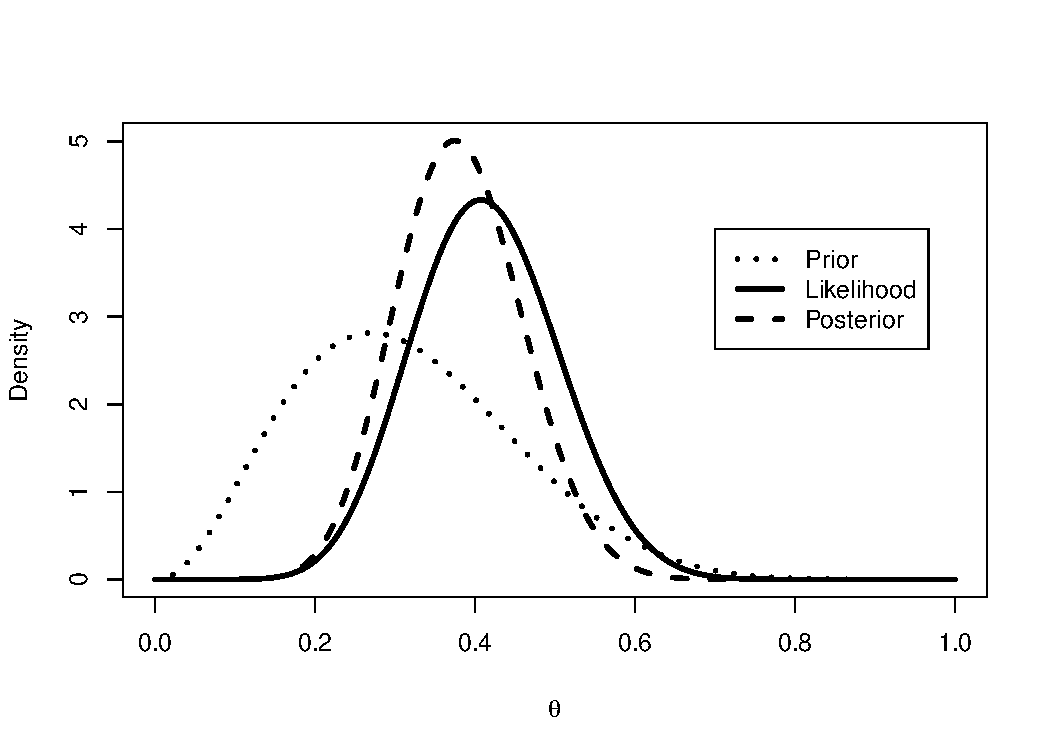
\includegraphics[width = .7\textwidth]{pics/sleep.pdf}
\caption{Likelihood $p(X|\theta)$ , Prior $p(\theta)$, and Posterior Distribution $p(\theta|X)$}
\label{fig:sleep}
\end{figure}


}

\end{frame}

%\frame{
%\frametitle{Multivariate Distributions}
%\begin{eqnarray*}
%\bX\mid \tth &\sim& N(\tth, \Sigma) \\ 
%\tth &\sim& N( \bmu, \Omega)
%\end{eqnarray*}
%\begin{eqnarray*}
%\pi(\tth \mid \bx ) & \propto &
%\exp\{ -1/2||\bx - \tth ||_\Sigma\}
%\exp\{ -1/2||\tth - \bmu ||_\Omega\}.
%\end{eqnarray*}

%Note that
%\begin{eqnarray*}
%&& (\bx - \tth)^T\Sigma^{-1} (\bx - \tth) 
%+ 
%(\tth - \bmu)^T\Omega^{-1} ( \tth -\bmu)  \\
%&=&
%\bx^T\Sigma^{-1} \bx
%+ \bmu^T\Omega^{-1} \bmu 
%+ \tth^T\Sigma^{-1}\tth -2\bx^T\Sigma^{-1}\tth +\bth^T\Omega^{-1} \bth \\
%&+&\bmu \Simga^{-1} \bmu - 2 \bmu^T \Sigma^{-1} \bth
%\end{eqnarray*}




}
%
%\frame{
%
%\begin{eqnarray*}
%\pi(\tth \mid \bx ) & \propto &
%\exp\{ -1/2||\bx - \tth ||_\Sigma\}
%\exp\{ -1/2||\tth - \bmu ||_\Omega\}.
%\end{eqnarray*}
%
%Note that
%\begin{eqnarray*}
%&& (\bx - \tth)^T\Sigma^{-1} (\bx - \tth) 
%+ 
%(\tth - \bmu)^T\Omega^{-1} ( \tth -\bmu)  \\
%\pause
%&=&
%\bx^T\Sigma^{-1} \bx
%+ \bmu^T\Omega^{-1} \bmu 
%+ \tth^T\Sigma^{-1}\tth -2\bx^T\Sigma^{-1}\tth +\tth^T\Omega^{-1} \tth \\
%\pause
%&+&\bmu \Sigma^{-1} \bmu - 2 \bmu^T \Sigma^{-1} \tth \\
%\pause
%&\propto& 
% \tth^T\Sigma^{-1}\tth -2\bx^T\Sigma^{-1}\tth +\tth^T\Omega^{-1} \tth 
% - 2 \bmu^T \Sigma^{-1} \tth \\
% \pause
% &\propto& \left\{ \tth - (\Sigma^{-1}+ \Omega^{-1})^{-1} \left(
% \Sigma^{-1}\bx+ \Omega^{-1}\tth
% \right)
% \right\}^T \times
% (\Sigma^{-1}+ \Omega^{-1})^{-1} \\
% \pause
% &\times&
% \left\{
%  \tth - (\Sigma^{-1}+ \Omega^{-1})^{-1} \left(
% \Sigma^{-1}\bx+ \Omega^{-1}\tth
% \right)
% \right\}  \impies
%\end{eqnarray*}
%$$\tth \mid \bx \sim N\left( (\Sigma^{-1}+ \Omega^{-1})^{-1} \left(
% \Sigma^{-1}\bx+ \Omega^{-1}\tth
% \right), 
%  (\Sigma^{-1}+ \Omega^{-1})^{-1} 
%\right )$$
%
%
%
%
%
%
%}

\frame{
\frametitle{What questions might we want to ask?}

\begin{itemize}
\item What is the posterior mean and variance? (Homework 1). 
\item Confidence intervals
\item If new data comes in, how do we predict whether these students are getting less than 8 hours of sleep?
\end{itemize}

Above questions we'll cover in Module 3!



}


%%Next time: Gibbs sampling. For more complicated model, we can not calculate the posterior in closed form, we must estimate it. How can we do this? 

\frame{
\frametitle{Coming up next}
Make sure you're feeling very familiar with R. See the Intro to Bayes Lab (with solutions). 
\vskip 1em
Module 2: Decision theory: how do we think about loss, risk (general decision making)?
\vskip 1em
%% TA's go through the first and second R labs. 
Wednesday: Lab with decision theory. 

%% TA's go through the sleep example in my slides. Show them how to plot the prior, likelihood, and posterior
%% for a beta. Then walk them through the sleep example in class. 
}




\end{document}